\section{Volume de billes (4 points)}


\begin{multicols}{2}
	

Noémie place des billes dans une éprouvette graduée.

\begin{questions}
	\question[1] Quelle est la valeur $V_1$ du volume du tas de billes dans l'éprouvette ? 
	
	\begin{solution}
		Le volume de billes mesuré dans la première éprouvette est $V_1 = 8 mL$. 
	\end{solution}
	
	\question[1\half] Elle verse de l'eau dans une éprouvette identique à la précédente. Puis elle verse l'eau dans l'éprouvette contenant les billes. Quel est le volume $V_2$ occupé par les billes ?
	\begin{solution}
		Le volume d'eau dans la deuxième éprouvette est 20 mL, celui mesuré dans la troisième qui contient l'eau et les billes est 25 mL.
		
		\begin{equation*}
			25 - 20 = 5
		\end{equation*}
		
		Donc le volume $V_2$ occupé par les billes est 5 mL.
	\end{solution}
	
	\question[1\half] Comment expliquer la différence entre le volume $V_1$ et le volume $V_2$.
	\begin{solution}
		La différence entre $V_1$ et $V_2$ correspond à l'espace entre les billes qui n'occupent pas entièrement les 8 mL. 
	\end{solution}
\end{questions}


\begin{center}
	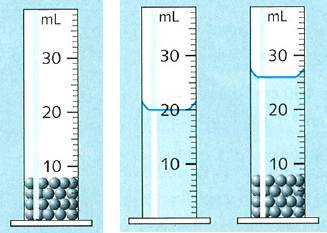
\includegraphics[scale=0.9]{img/billes}
\end{center}
\end{multicols}